\section{El concepto de co-creación de valor} 

Para poder arrojar luz al término de co-creación de valor, se han de definir los conceptos de valor y de valor añadido. En el anexo \ref{anexo:1} se puede encontrar más información al respecto. Por un lado, para el autor Sawhney (2006), el valor viene establecido por el valor percibido por el cliente de un producto o servicio en relación con el coste total que los consumidores pagan por el. Por lo tanto, se puede definir el valor añadido como el valor creado a lo largo del proceso, es decir, desde el vendedor hasta el consumidor, teniendo en cuenta la cantidad y el precio que están dispuestos a invertir en un producto o servicio que no sólo cubra las necesidades, si no también que aporte algún factor añadido (Brandenburguer y Harbone, 1996). 


En lo que se refiere a la co-creación de valor, en primer, lugar hay que destacar que las interacciones directas entre los consumidores y las compañías constituyen un factor fundamental en la co-creación de valor, ya que promueven la participación activa del cliente en todos los aspectos, incluyendo la búsqueda de información, la configuración de productos y servicios y el consumo (Prahalad y Ramaswamy, 2004).

Otro de los aspectos fundamentales es el giro de 180 grados en a mentalidad de los clientes. En las últimas décadas el cliente se ha implicado en el proceso de co-creación de valor cambiando su rol participativo dentro de las compañías. De este modo, adquiere un papel cada vez más activo. 

Debido a que el término de co-creación es relativamente novedoso, la literatura todavía se encuentra en una fase de desarrollo, pero en los últimos años si que se ha podido apreciar una insistencia mayor por parte de los autores en abordar esta temática, por ejemplo, investigadores como Vargo y Lusch; Grönroos, O´Hernd y Rindfleisch, Prahalad y Ramaswamy entre los más destacados y por lo tanto los que se van a tomar como referencia a lo largo de este capítulo  exponiendo sus principales ideas.

La co-creación de valor es un reflejo de que el valor no lo crea la empresa en solitario, sino que es necesaria la interacción con su entorno, considerando al cliente el principal creador de valor. Hoy por hoy, los clientes están más informados y educados y por lo tanto también son más selectivos, exigentes y tienen una mayor capacidad de elección. La evolución del perfil del consumidor es patente, ya que demanda una mayor generación de valor por parte de las empresas. Este hecho influye en las organizaciones de una forma muy significativa porque la creación de valor se ha vuelto necesaria para la supervivencia de estas (Hunt et al., 2012).

Estudios recientes demuestran que el valor generado puede favorecer no sólo a la satisfacción del cliente sino también en los resultados empresariales (Guenzi y Troilo, 2007). A continuación, se van a exponer las definiciones de los tres autores más relevantes de este capítulo, Prahalad y Ramaswamy; Vargo y Lusch y Grönroos.

Para Prahalad y Ramaswamy, (2004) la co-creación implica la creación de valor conjunta entre el proveedor y el cliente donde se requiere la construcción de experiencias y la resolución de problemas con un esfuerzo combinado de todas las partes que componen la relación comercial. 

Vargo y Lusch (2004) ratifican la definición anterior considerando la co-creación como una forma de aumentar el valor tanto para los clientes como para los proveedores de bienes o servicios. 

Para Grönroos (2006), la co-creación de valor son las actividades que llevan a cabo las partes implicadas en el proceso interactivo destinadas a contribuir valor y se da por una o por  ambas partes, o si se ampliase el modelo, por todas las partes.

Hay que tener en cuenta que en los procesos de co-creación de valor pueden existir en comunidades de consumidores. Yi y Gong (2012) defienden dos grupos: la participación individual y la participación de comunidades de consumidores. 

\begin{figure}[!h]
	\caption{Evolución de las relaciones entre empresa y consumidor}
	\centering 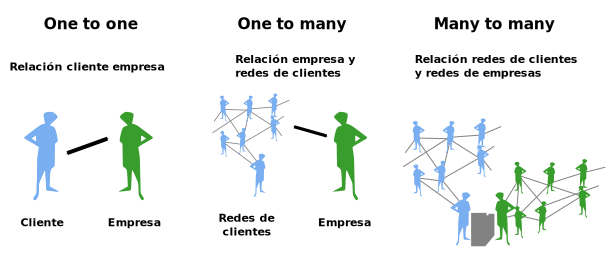
\includegraphics[width=150mm]{capitulos/graficos/oneMany} 
	\label{fig:oneMany} 
	
		\footnotesize
		Fuente: Adaptado de Gummensson, 2004, p. 3.
\end{figure}

En cambio, Prahalad y Ramaswamy (2004), Blasco, (2014) y Gummensson (2004), establecen una escala con tres niveles, dependiendo del número de clientes y la complejidad de la interacción entre la/s empresa/s y el/los cliente/s. En la figura  \ref{fig:oneMany}, se puede apreciar la evolución de estas relaciones surgidas a lo largo del siglo XX (Gummensson, 2004) que son las siguientes:

\begin{itemize}
	\item \emph{One to one} o interacción entre la empresa y el cliente. La contribución \emph{one to one} es la más tratada en la literatura ya que es la forma más sencilla de arrojar luz sobre la interacción individual en la comercialización (Gummensson, 2004).


	\item \emph{One to many} o interacciones entre la empresa y comunidades de clientes. Es un proceso, mediante el cual la empresa transmite informaciones, contenidos, sugerencias, etc. También se puede dar el caso de que la empresa permita interactuar a las comunidades de consumidores entre si (Hoffman y Novak, 1995). Además, la heterogeneidad de los clientes hace que la empresa tenga que adaptarse al amplio abanico de reacciones de estos. Y por lo tanto, la compañía tiene que tener en cuenta que se pueden dar numerosos casos distintos de co-creación de valor (Gummensson, 2004).

 	\item \emph{Many to many} o interacciones llevadas a cabo entre redes de empresas y comunidades de consumidores. La contribución de \emph{many to many} es la más compleja y aborda todo el contexto de un modelo mucho más complejo . Surgió en el año 2000 con el objetivo de describir, analizar y utilizar las propiedades de las nuevas redes de comercialización para poder dar un carácter personalista y poder co-crear valor a través de la interacción (Gummensson, 2004).

\end{itemize}


 Las dos relaciones más comunes de las tres mencionadas anteriormente según Gummensson (2004), son \emph{one to one} y \emph{many to many}. En el cuadro \ref{tab:diferencias} se pueden apreciar algunas de las diferencias entre estas dos propuestas.

\begin{table}[h]
    \caption {Diferencias entre one to one y many to many}
	\label{tab:diferencias}
	\setlength\extrarowheight{5pt}
	
	\begin{tabular}{p{7cm} p{7.5cm}}
	\toprule
	One to one                                           & Many to many                                                                             \\ 
\midrule
	La empresa identifica al consumidor.                 & Las redes de empresas identifican a las redes de consumidores.                           \\
	La empresa diferencia a un consumidor de otro.       & Las redes de empresas se diferencian a través de sus propias relaciones.                 \\
	La empresa interactua con el consumidor.             & Las redes de empresas interactúan con las redes de consumidores a través de otras redes. \\
	La empresa aprende a relacionarse con su consumidor. & Las redes de empresas aprenden a relacionarse a través de redes.                         \\ 
	\bottomrule
	\end{tabular}

	\center
	\footnotesize
	Fuente: adaptado de Gummensson, 2004. p: 3
\end{table}


 Por lo tanto, se puede decir que \emph{one to one} tan sólo abarca la relación individual de una transacción entre una única empresa y un único cliente y en cambio, \emph{many to many} es mucho más compleja y trata de abordar la red de relaciones que tienen las empresas y la red de relaciones que también tienen los consumidores utilizando otra serie de redes para conectar ambas entre si.

Un ejemplo de las redes de relaciones de consumidores son las comunidades Web. En la figura \ref{fig:WomGebauer}, se puede apreciar el modelo conceptual creado por Gebauer, Füller y Pezzei (2013) donde se observa el comportamiento que los usuarios pueden adoptar a la hora de co-crear valor a través de una comunidad Web. Los comportamientos de los clientes pueden ser dos:

\begin{itemize}
	\item \emph{WOM}. Es el boca a boca o también conocido como boca a oreja. Las siglas se corresponden con las palabras inglesas: Word of Mouth.
	\item \emph{WTP}. Son las siglas inglesas \emph{Willingness To Pay}, que se traduce como lo que el cliente está dispuesto a pagar por un producto o servicio.

\end{itemize}

\begin{figure}[!h]
	\caption{El modelo conceptual del comportamiento por parte de los usuarios en las comunidades de innovación online}
	\centering 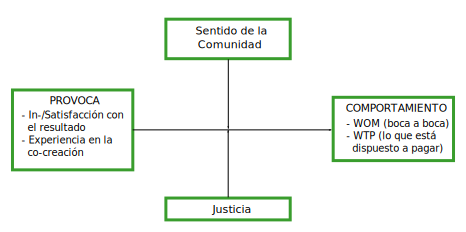
\includegraphics[width=130mm]{capitulos/graficos/WomGebauer} 
	\label{fig:WomGebauer} 
	
		\footnotesize
		Fuente: Gebauer, Füller y Pezzei, 2013, p. 1522.
\end{figure}


Tradicionalmente, se afirmaba que mediante el boca a boca de un consumidor insatisfecho, este usuario transmitía su sentimiento de decepción hacia esa marca a cinco personas de su entorno. Sin embargo, la situación actual es muy diferente, ya que la magnitud es mucho mayor con el desarrollo de las redes sociales (Gebauer, Füller y Pezzei, 2013). Un claro ejemplo es Facebook, esta red social tiene una media mensual de un billón de usuarios activos que a su vez están conectados a 130 amigos de media (Facebook, 2014). Por lo tanto, las opiniones publicadas en las redes sociales, que pueden estar abiertas al público y no sólo al círculo cercano del usuario, tienen un efecto boca a boca mucho más potente y trascendente que en el propio medio social del individuo. Por lo tanto, la co-creación de valor, no siempre es positiva y se puede dar el caso de que la co-creación de valor sea negativa. Se puede encontrar más información respecto a este tema en el anexo \ref{anexo:2}.

En lo que se refiere al proceso de co-creación de valor entre las empresas y los clientes, Yi y Gong (2012) proponen ocho pasos en el sector servicios. A continuación se exponen junto con un ejemplo del sector hotelero:

\begin{enumerate}
	\item \emph{La búsqueda de información}. El huésped potencial puede revisar opiniones de otros huéspedes a través de Tripadvisor.
	\item \emph{El intercambio de información}. El huésped puede reportar problemas al hotel y puede comunicar a otros clientes si se solucionaron con eficacia o no.
	\item \emph{El comportamiento responsable}. Seguir las indicaciones del personal de cocina a la hora del desayuno, comida o cena.
	\item \emph{La interacción personal}. Los empleados deben de adoptar una postura de respeto permanente hacia el cliente.
	\item \emph{Feedback de los clientes}. Los huéspedes deben reportar siempre cualquier problema surgido a lo largo de la estancia y posteriormente pueden realizar una encuesta de calidad para dar una valoración del hotel.
	\item \emph{Promoción}. Es muy importante que los clientes queden satisfechos para que puedan promocionar y recomendar la empresa a desconocidos, familiares y amigos. Es una herramienta de marketing muy importante como se ha podido apreciar en la figura \ref{fig:WomGebauer}, por lo que hay que promover la satisfacción de los clientes.
	\item \emph{Ayuda}. Las opiniones de los huéspedes son muy valiosas para la compañía hotelera porque les ayuda a integrar nuevas herramientas de co-creación de valor en un futuro.
	\item \emph{Tolerancia}. Durante el check in y el check out pueden surgir problemas informáticos, en la gestión de cobros, etc. y el huésped ha de aprender a ser paciente.

\end{enumerate}


Por lo tanto, Yi y Gong (2012) dan importancia a la conducta que adquieren los clientes. Los procesos de co-creación de valor, deben ayudar a los directivos a la hora de elegir nichos de mercado. De este modo, si una empresa evalúa periódicamente las actividades que desarrollan los clientes dentro de la corporación, éstos estarán a su vez más dispuestos a involucrarse en eventos propuestos por la empresa para la co-creación de valor y por lo tanto podrán fidelizarse con la compañía.

\section{Los procesos de co-creación de valor}
\label{section:procesosCocreacion}

A lo largo de literatura dedicada al proceso de co-creación de valor, los autores han decidido centrarse en mayor medida en la relación entre cliente y empresa. Dentro de esta vertiente, Blasco (2014) diferencia dos enfoques: 

\begin{itemize}
	\item Los procesos de co-creación de valor que se pueden dar entre empresa y cliente (Prahalad y Ramaswamy, 2004; Payne et al., 2008), y 
	\item Los procesos de co-creación de valor como una oportunidad de desarrollo de nuevos productos y/o servicios (O’hern y Rindfleisch, 2010). 

\end{itemize}

Los procesos de co-creación de valor como una oportunidad de desarrollo de nuevos productos y/o servicios, dada su poca relación con el objetivo del trabajo no se va a desarrollar en el presente capítulo; se puede encontrar información al respecto en el anexo \ref{anexo:3}. 
A continuación se va a arrojar luz acerca de la co-creación de valor desde el punto de vista del intercambio de información entre la empresa y el cliente. 

\subsection{La participación de la empresa y el cliente en el proceso de creación de valor}

Es destacable que a la hora de producir un servicio se distingan tres formas dependiendo del grado de participación que se le permita al consumidor (Blasco, 2014) (ver figura \ref{fig:procesosCocreacionPayne}):

\begin{itemize} 
	\item Producción completa de la empresa. 
	\item Producción conjunta (relación empresa-cliente). 
	\item Producción del cliente. 
\end{itemize}


\begin{figure}[!h]
	\caption{El proceso de co-creación de valor cliente-empresa}
	\centering 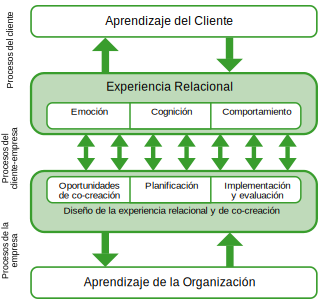
\includegraphics[width=100mm]{capitulos/graficos/procesosCocreacionPayne} 
	\label{fig:procesosCocreacionPayne} 
	
		\footnotesize
		Fuente: Payne, Storbacka y Frow, 2008, p. 96.
\end{figure}

Payne et al. (2008), definen el proceso de creación de valor del cliente como una serie de actividades llevadas a cabo por el usuario para lograr un objetivo particular. El aspecto clave para estos autores, es que la capacidad del cliente para co-crear valor depende de la cantidad de información, de los conocimientos, de las habilidades y de otros recursos operantes que pueden utilizar. Si una empresa quiere mejorar su competitividad, tiene que desarrollar su capacidad y utilizar los recursos de los que dispone de la manera más eficiente y eficaz. Estos autores diferencian tres tipos de etapas a lo largo de este proceso (ver figura \ref{fig:procesosCocreacionPayne}) que se van a explicar a continuación (Payne et al., 2008):


\begin{enumerate} 
	\item \emph{El proceso de co-creación de valor para el cliente}. Los clientes están involucrados en un proceso cognitivo donde realizan juicios en base a sus experiencias de consumo, es decir, a partir de las emociones, de los aspectos contextuales, simbólicos y no utilitarios del propio consumo. En este enfoque, se espera que el cliente esté dispuesto a obtener el conocimiento suficiente para evaluar los beneficios y los sacrificios que conllevan la adquisición del producto o el disfrute del servicio. Si el cliente acepta este reto, las actividades que se han de llevar a cabo son: la búsqueda de información, la evaluación de opciones disponibles y decidir si debe o no comprar un producto o servicio en particular (Payne et al., 2008). Desde este enfoque, se considera que el valor no reside en el momento de la compra o disfrute del bien o servicio, sino en la experiencia de consumo a través de fantasías, sentimientos y diversión. De este modo, Payne et al. (2008), consideran a los clientes como \emph{hacedores y pensadores} de co-creación de valor (ver figura \ref{fig:procesosCocreacionPayne}).
	\item \emph{El proceso de co-creación de valor para la empresa}. Se ha de tener en cuenta el punto anteriormente descrito ya que los clientes crean valor con el apoyo de la empresa. En la figura \ref{fig:procesosCocreacionPayne} se puede apreciar que la empresa participa en la co-creación de valor a través del diseño y la entrega de experiencias al cliente facilitando a su vez el aprendizaje de la compañía. Según Payne et al. (2008), esto implica revisar constantemente las oportunidades que la compañía ofrece a la hora de co-crear, planificar, dar soluciones a los clientes, gestionar los recursos humanos de los que se dispondrán y poner a prueba las medidas diseñadas para los clientes por si no se se están realizando las propuestas de valor adecuadas. Por lo que, partiendo de los procesos de aprendizaje del cliente, una empresa puede diseñar sus propios procesos para aproximarse cada vez más a los de sus clientes. La implementación de este proceso puede desembocar en mejores oportunidades en el proceso de co-creación de valor. 
	\item \emph{El proceso de co-creación de valor entre empresa y cliente}. Se trata de interacciones bidireccionales que se dan entre el cliente y la empresa. Payne et al. (2008) las denomina puntos de contacto. Pueden darse por iniciativa de la propia empresa o por parte del cliente. En la figura \ref{fig:procesosCocreacionPayne}, las interacciones están representadas a través de las flechas situadas entre el cliente y la empresa. Un ejemplo aplicado a la parte empírica expuesta en el capítulo \ref{section:parteEmpirica}, podría ser una campaña de marketing por parte del la empresa hotelera ofreciendo estancias en hoteles a precios reducidos. En algunos casos, la comunicación puede darse por una parte, por ejemplo gracias al envío de publicidad del hotel a los huéspedes fidelizados. Aun así, Payne et al. (2008) opina que ambas partes participan en el proceso porque que la lógica del servicio (Grönrros, 2004) apoya la teoría de que el diálogo es creciente entre ambas partes.

\end{enumerate}

Para finalizar con este epígrafe centrado en los procesos de co-creación de valor, se va a presentar la figura \ref{fig:metasMaram} donde se puede apreciar las relaciones que tanto empresa como cliente han de desarrollar en los procesos productivos para alcanzar la meta de la co-creación de valor y poder obtener clientes fieles, que se impliquen en las tareas de marketing y publicidad a través del boca a boca (Maram, 2013).

\begin{figure}[!h]
	\caption{Pasos para alcanzar la co-creación de valor}
	\centering 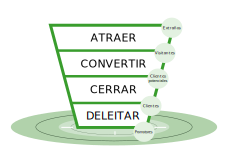
\includegraphics[width=110mm]{capitulos/graficos/metasMaram} 
	\label{fig:metasMaram} 
	
		\footnotesize
		Fuente: Maram, 2013
\end{figure}

\section{Las teorías asociadas a la co-creación de valor}

En el presente epígrafe, se van a describir las principales teorías surgidas sobre la co-creación de valor desarrolladas hasta el momento. En la figura \ref{fig:esquema} se aprecia un esquema de las tres diferentes ramas que se van a asumir acerca de la co-creación de valor y los autores creadores o defensores de éstas. Se va a seguir el modelo de segregación en tres vertientes de los autores Chen et al. (2012).

\begin{figure}[!h]
	\caption{Esquema de las teorías de co-creación de valor}
	\centering 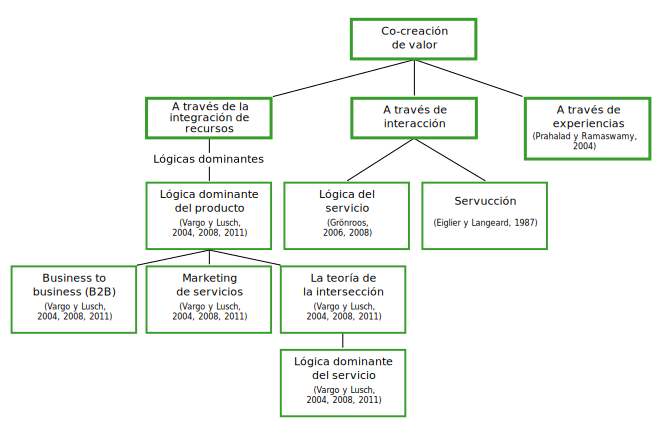
\includegraphics[width=150mm]{capitulos/graficos/esquema} 
	\label{fig:esquema} 
	
		\footnotesize
		Fuente: elaboración propia
\end{figure}

Como se puede apreciar en la figura \ref{fig:esquema}, Vargo y Lusch son defensores de la lógica dominante del servicio que parte de las premisas de la lógica dominante del producto; Grönroos apoya la lógica del servicio; Eigler y Langeard desarrollan la teoría de la servucción; y por último, Prahalad y Ramaswamy defienden las relaciones personalizadas entre empresa y cliente para que éste último pueda interaccionar con el entorno empresarial y crear experiencias personalizadas. 

\subsection{La co-creación de valor a partir de la integración de recursos}

\subsubsection{Las lógicas dominantes}

El término de lógica dominante hace referencia a las pautas que desarrolla una empresa para obtener beneficios. En la lógica dominante se describen las normas y las creencias culturales que la empresa ha desarrollado en su camino al éxito o al fracaso. Aitken, et. al. (2006) definen la lógica dominante como un pensamiento común basado en las estrategias de diferentes empresas.

\paragraph{De la lógica dominante del producto a la lógica dominante del servicio}
\label{section:logicasDominantes}

La lógica dominante del producto (LDP), no distingue entre bienes tangibles e intangibles y su esencia es el intercambio económico de unidades de producción que tienen el valor intrínseco en si mismo. La producción y el desarrollo del bien se realiza sin el cliente (Vargo y Lusch, 2008). La figura \ref{fig:valorUso} refleja estas diferencias marcadas por Vargo y Lusch (2004) entre el proceso de co-creación de valor en el intercambio (LDP) y el proceso de co-creación de valor en el uso (LDS). En este último, la variable más trascendente es la experiencia de valor acumulada en uso por parte del cliente, ya que en este modelo, el cliente tiene que participar en el proceso de co-creación de valor. 

\begin{figure}[!h]
	\caption{Comparación del proceso de co-creación en el modelo de valor en el intercambio y en el modelo de valor en uso}
	\centering 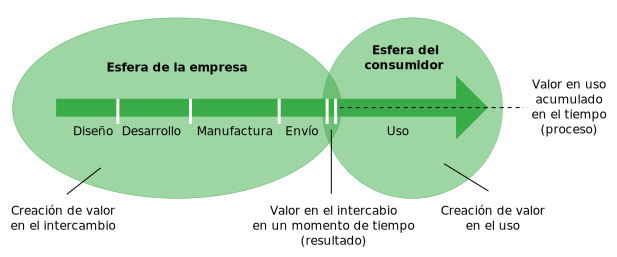
\includegraphics[width=150mm]{capitulos/graficos/valorUso} 
	\label{fig:valorUso} 
	
		\footnotesize
		Fuente: Grönroos y Voima, 2011, p. 4.
\end{figure}

Para poder comprender esta evolución de teorías, en la figura \ref{fig:evolucion} se van a delimitar las fechas en las que surgen cada una de las teorías. Los tres enfoques surgidos a partir de la LDP, son conceptos definidos en el anexo \ref{anexo:4}.

\begin{figure}[!h]
	\caption{Evolución de la lógica dominante}
	\centering 
\includegraphics[width=150mm]{capitulos/graficos/evolucion} 
	\label{fig:evolucion} 
	
		\footnotesize
		Fuente: elaboración propia a partir de Vargo y Lusch, 2008
\end{figure}

Como se puede observar en la figura \ref{fig:evolucion}, el concepto lógica dominante del servicio (LDS) surge por primera vez en la obra de Smith del año 1776, se desarrolló a lo largo de un siglo atravesando también la revolución industrial y llegó hasta los años 60 acumulando un amplio conocimiento acerca de la economía (Vargo y Lusch, 2008). Desde las raíces de esta teoría, se consideró que la empresa creaba un producto con un valor añadido intrínseco y el cliente destruía ese valor a través del consumo. Pero como bien se ha mencionado, a partir de 1960 la mentalidad empresarial sufrió un cambio y esta teoría comenzó a ser cuestionada, dando lugar a la creación de subdisciplinas. El nacimiento de éstas se debe a la limitación de la LDP para dar respuesta a la creación de valor y al intercambio entre otros factores, ya que la LDP solo se refiere a la distribución de productos (Vargo y Lusch, 2008).


A continuación, se van a exponer las características más importantes de la lógica dominante del servicio (LDS) y de la lógica dominante del producto (LDP). Se explican al mismo tiempo ya que Vargo y Lusch (2004) las tratan conjuntamente.

Se puede afirmar que la LDS surgió de las limitaciones que la LDP tenía para el concepto de servicio. Tanto Vargo y Lusch (2004), como Grönroos  (2006), coinciden en que los servicios también forman parte de la teoría de la lógica dominante del producto de una forma secundaria, pero para poder abarcar más elementos Vargo y Lusch (2004) crearon la lógica dominante del servicio. Esta nueva rama, abarcaba conceptos de procesos de comercialización para la empresa que la LDP no contemplaba tales como las relaciones a largo plazo, la calidad percibida por el cliente, las relaciones entre usuario y empresa, la transparencia, los enfoques hacia el intercambio y la sostenibilidad entre otros. Estos nuevos conceptos incluidos en la LDS, permitieron a Vargo y Lusch, desarrollar este nuevo modelo con variaciones en la forma de crear valor y la forma de intercambiar el servicio, como por ejemplo la calidad percibida y los recursos humanos dispuestos por la empresa. 

Según establecen Vargo y Lusch, (2011) la lógica dominante del servicio es una lógica \emph{de y para} el mercado, la sociedad y la comercialización. Esta nueva concepción centrada en el servicio, se ve reflejada en que la co-creación de valor es la integración de valor en el propio contexto teniendo en cuenta los resultados y los recursos de la empresa. Por ejemplo, como un huésped utiliza los recursos disponibles del hotel (Vargo y Lusch, 2008). Por lo tanto, estos autores establecen que la integración predeterminada de recursos en un proceso co-creativo es un medio de creación de valor.

Otro de los obstáculos de la LDP era el léxico. La primera columna del cuadro \ref{tab:evolucionLexica} está referida a la LDP, y se trata de un léxico basado en la economía de la primera década de 1800 que fue aceptado y utilizado al menos hasta aproximadamente el año 1980. Alrededor de 1980, surgió una grieta en el léxico provocada por una transición de la comercialización del servicio al marketing relacional y los recursos de intercambio y competencia, entre otros (Vargo y Lusch, 2004). Algunas de estas palabras llevan connotaciones muy específicas y se encuentran encasilladas en una lógica concreta y a menudo son incompatibles (Vargo y Lusch, 2004). Por ejemplo, productor y consumidor; bienes y servicios; demanda y oferta; etc. El léxico que surge para la LDS es más cercano y agradable para el cliente como por ejemplo los términos diálogo, proposiciones de valor, soluciones, etc. Vargo y Lusch (2004) afirman que todavía no se ha desarrollado plenamente todo el léxico que se debería para la LDS, por ello, plantean seguir desarrollando la LDS. 

\begin{table}[h]
    \caption {Evolución del léxico en las lógicas dominantes}
	\label{tab:evolucionLexica}
	\setlength\extrarowheight{5pt}
	
	\begin{tabular}{p{5cm} p{5cm} p{5cm}}
	\toprule
	LDP                               & Transición                            & LDS                              \\ \midrule
	Bienes                            & Servicios                             & Servicio                         \\
	Productos                         & Ofertas                               & Experiencias                     \\
	Características/atributos         & Beneficio                             & Soluciones                       \\
	Valos añadido                     & Co-producción                         & Co-creación de valor             \\
	Beneficio máximo                  & Ingeniería financiera                 & Aprendizaje financiero           \\
	Precio                            & Entrega de valor                      & Proposición de valor             \\
	Sistemas de equilibrio            & Sistemas dinámicos                    & Sistemas complejos de adaptación \\
	Red de creación de valor          & Cadena de valor                       & Red de co-creación de valor      \\
	Fomento                           & Marketing de comunicaciones integrado &                                  \\
		                              &                                       & Diálogo                          \\
	Mercado orientado a los productos & Mercado orientado al mercado          & Mercado orientado al servicio    \\ \bottomrule
	\end{tabular}
	
	\center
	\footnotesize
	Fuente: Vargo y Lusch, 2004. p. 286
\end{table}


Esta evolución lingüística también afecta a la forma de entender la co-creación de valor. Por ello, Vargo y Lusch (2008) establecen tres importantes diferencias:

\begin{enumerate} 
	\item La LDP afirma que el valor de bienes y servicios está intrínseco en el propio bien. En cambio, la LDS considera que el servicio es el proceso por el que la empresa hace algo para el cliente sin hacer referencia a los bienes que intervienen en el intercambio. Esto quiere decir que en la LDS los bienes siguen teniendo un papel importante aunque no sean mencionados (Vargo y Lusch, 2008). 
	\item El tratamiento de los elementos. La LDP, considera que los servicios tienen una categoría inferior a la de los bienes fabricados, y la LDS, en cuanto a la co-creación de valor, considera que es un proceso relacional de intercambio de servicio por servicio. Este intercambio, implica que tanto empresa como cliente son co-creadores y beneficiarios de valor, y deben considerarse como integradores de recursos (Vargo y Lusch, 2011). 
	\item La diferencia de léxico entre servicios y servicio: 
		\begin{itemize} 
			\item Los servicios. Son unidades de \emph{output} (Vargo y Lusch, 2004). Para Grönroos (2004), son procesos de una serie de actividades en las que la empresa utiliza unos recursos determinados cuando interacciona con el cliente. Se relaciona con la LDP.
			\item El servicio. Se trata de un proceso de \emph{algo para alguien} (Vargo y Lusch, 2004). Se relaciona con la LDS.

			De este modo, el uso del término servicio en singular en contra a los servicios que plantea la LDP, es intencional y no trivial (Vargo y Lusch, 2008). Para Vargo y Lusch (2004) uno de los errores fundamentales de la LDP es que el servicio es considerado como un tipo especial de bien intangible.
			\end{itemize}

\end{enumerate}

Por otro lado, en la LDS el proceso de co-creación de valor recíproco es un proceso continuo de integración de recursos que pueden ser de dos tipos (Vargo y Lusch, 2006):

\begin{itemize} 
			\item Los recursos operandos. Vargo y Lusch (2008) los definen como los recursos sobre los cuales se realiza una operación o un acto para producir un efecto, es decir, se trata de recursos estáticos e inertes que necesitan de otros recursos dinámicos para que sean útiles. Algunos ejemplos son los recursos naturales, bienes, materiales tangibles, etc. (Vargo y Lusch, 2008).
			\item Los recursos operantes o dotación de recursos. Son los recursos capaces de afectar sobre los recursos operandos ya que se refieren a las habilidades, el conocimiento, la imaginación, las emociones y las experiencias de los clientes. Por lo tanto, estos recursos también afectan a la co-creación de valor. Se puede ampliar el modelo co-creativo incluyendo las interacciones entre empresas, clientes y \emph{stakeholders} (Vargo y Lusch, 2011). Como conclusión, Vargo y Lusch (2008) establecen que todo el entorno social y económico integra recursos de un tipo u otro.

\end{itemize}

Teniendo en cuenta la integración de recursos mencionada en el párrafo anterior, se puede observar la figura \ref{fig:LDSVargoLusch} que refleja el proceso de co-creación de valor en la lógica dominante del servicio. En ella se muestra cómo interaccionan los clientes con la empresa mediante los recursos internos y externos que se proporcionan, teniendo en cuenta también los agentes que podrían considerarse como resistencias a la co-creación de valor. Hasta que estas resistencias u obstáculos sean superados e integrados por la empresa, se continuará utilizando el mismo sistema de interacción entre el cliente y la empresa para co-crear valor (Lusch y Vargo, 2007).

\begin{figure}[!h]
	\caption{El proceso de co-creación de valor en la lógica dominante de los servicios}
	\centering 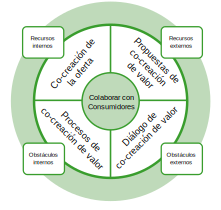
\includegraphics[width=100mm]{capitulos/graficos/LDSVargoLusch} 
	\label{fig:LDSVargoLusch} 

	\footnotesize
		Fuente: Vargo y Lusch, 2008, p. 4.
\end{figure}

En resumen, el paso natural de la LDP hacia la LDS propone los siguientes cambios (Vargo y Lusch, 2008) (ver cuadro \ref{tab:transicion}): 

\begin{enumerate} 
			\item Del pensamiento de producción de bienes y servicios a un proceso de ayuda al cliente para facilitar el desarrollo de la co-creación de valor. 
			\item Concebir el valor como un bien producido y vendido a verlo como una variable co-creada en conjunto con el cliente y el entorno. 
			\item Considerar al cliente como parte de la empresa y no como un ente aislado.
			\item Incluir los recursos operantes intangibles como el conocimiento y las habilidades a los recursos operandos de la empresa como pueden ser los recursos naturales. 
			\item Concebir a los clientes como fuente de información y recursos. 
			\item El cambio de mentalidad de que prime la eficiencia a que aumente esa eficiencia a través de la eficacia. 

\end{enumerate}

\begin{table}[h]
    \caption {Transición de la LDP a la LDS.}
	\label{tab:transicion}
	\setlength\extrarowheight{5pt}
	
	\begin{tabular}{p{7cm} p{7.5cm}}
	\toprule
	LDP                                                      & LDS                                                                          \\ \midrule
	Producir bienes o servicios.                             & Ayudar a los clientes en los procesos de co-creación de valor.               \\
	El valor se halla en los bienes o servicios producidos.  & Los clientes no son entidades aisladas si no que forman parte de la empresa. \\
	Los recursos principales de la empresa son los operandos. & Los recursos principales de la empresa son los operantes.                    \\
	Los clientes son el objetivo.                            & Los clientes son recursos.                                                   \\
	Prima la eficiencia.                                     & Prima la eficiencia a través de la eficacia.                                 \\ \bottomrule
	\end{tabular}

	\center
	\footnotesize
	Fuente: Vargo y Lusch, 2008. p. 5.
\end{table}


Estos cambios implican una remodelación de valores empresariales que facilitan la co-creación de valor conjuntamente. Es decir, se trata de un intercambio entre empresa, cliente y entorno. 

Como conclusión, se puede afirmar que el fin de la LDP es la reciprocidad, es decir, el momento en el que se presta el servicio ha de hacerse \emph{para y con el cliente} con el objetivo de obtener un intercambio de servicio por servicio.  Los productos pueden aparecer en este intercambio pero como complementos y en segundo plano. Los elementos participantes fundamentales son el conocimiento y las habilidades que la compañía emplea para la creación de valor (Vargo y Lusch, 2004). Por tanto, queda patente que en la teoría de la LDS, la co-creación de valor se centra en el hecho de que el cliente siempre participa activamente en el proceso de co-creación de valor, implicándose hasta tal punto de emplear sus propios recursos operantes además de aprovechar los recursos facilitados por la empresa (Vargo et al., 2010). En estudios paralelos de Vargo, Maglio y Akaka (2008) se propone la co-creación de valor como un proceso más complejo en el que se incluyen agentes como los \emph{stakeholders}, agencias gubernamentales, etc. No se va a entrar en más detalle por la complejidad que supone este modelo.

\subsection{La co-creación de valor a través de la interacción}

En este epígrafe se van a explicar dos teorías que defienden que el intercambio de valor se produce en el momento en el que la empresa y el cliente interaccionan entre sí, por ello, la empresa debe procurar instaurar sistemas que permitan estas interacciones. Las dos teorías más relevantes de co-creación de valor a través de la interacción son (Blasco, 2014):

\begin{itemize} 
    \item El modelo de servucción (Eiglier y Langeard, 1975, 1976). 
    \item La lógica del servicio (Grönroos, 2006, 2008). 
\end{itemize}

Como se puede apreciar en la figura \ref{fig:procesoProductivoEiglier}, la diferencia fundamental entre la producción de productos y la producción de servicios está en que en el \emph{input} existen otros elementos. En los servicios, el cliente es simultáneamente el productor y el consumidor, es decir, la entrada y la salida del proceso productivo es el cliente. Esto ocurre porque el consumidor es quien ha disfrutado del servicio y ha sido al mismo tiempo co-productor. En cambio, en la producción de un bien tangible, existe una transformación de recursos y por lo tanto, el \emph{input} y el \emph{output} son diferentes. Por ello, es necesario incorporar esta herramienta de diseño de servicios, al departamento de calidad de empresas dedicadas a los servicios (Eiglier y Langeard, 1976). 

\begin{figure}[!h]
	\caption{Diferencias en el proceso productivo del servicio y del producto}
	\centering 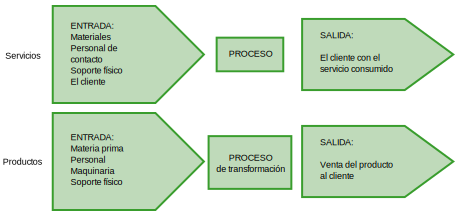
\includegraphics[width=150mm]{capitulos/graficos/procesoProductivoEiglier} 
	\label{fig:procesoProductivoEiglier} 

	\footnotesize
		Fuente: Adaptado de Lilian, 2004, p. 5.
\end{figure}

En primer lugar, se describirá la teoría de Eigler y Langeard diseñada en los años 80. Y en segundo lugar, la teoría desarrollada por la escuela nórdica, más concretamente por Grönroos sobre la lógica del servicio y el marketing interactivo que se ha creado en la primera década del año 2000.

\subsubsection{La servucción}

Eiglier y Langeard, (1976) definen servucción como la organización sistemática y coherente de todos los elementos físicos y humanos que surgen de la relación entre el cliente y la empresa y que es necesaria en la prestación de servicios, donde las características comerciales y los niveles de calidad que se van a ofrecer han sido determinados por la empresa.

Cuando la empresa establece su plan de prestación de servicios, tiene que tener una serie de factores que van a influir en este proceso y que han de desarrollarlos con sumo cuidado. Por ejemplo, la gestión de los procesos de trabajo, las capacidades personales, el flujo de clientes, etc. Puede considerarse un reto para la empresa ya que pone de manifiesto la creatividad y a la precisión de la que disponen, teniendo en cuenta todos los elementos subjetivos que se pueden dar en el comportamiento del cliente. Por ejemplo, las relaciones establecidas con el personal prestador del servicio, las expectativas, los deseos, las variaciones y las percepciones decisivas del cliente, etc. Hay que tener en cuenta un aspecto fundamental, y es que \emph{sin cliente no existe el servicio} (Eiglier y Langeard, 1976). Por ejemplo, si el cliente no ocupa la habitación de un hotel solo se daría la capacidad ociosa de servicio, pero no el servicio en si. 

\begin{figure}[!h]
	\caption{La servucción: empresa, cliente y entorno según Eiglier y Langeard}
	\centering 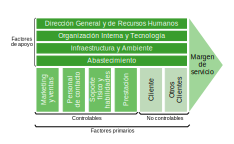
\includegraphics[width=140mm]{capitulos/graficos/servuccion} 
	\label{fig:servuccion} 

	\footnotesize
		Fuente: Alonso, 2008, p. 89.
\end{figure}

A continuación se va a dar sentido a la figura \ref{fig:servuccion} a través de ejemplos para un hotel, que es el tema a tratar en el capítulo \ref{section:parteEmpirica}.

Los factores principales que pueden ser controlables por la empresa son (Eiglier y Langeard, 1976):

\begin{itemize} 
			\item El marketing y las ventas. No se da con frecuencia, pero algunos ejemplos son: promocionar un nuevo alimento en el desayuno, una ropa de cama más confortable, etc. 
			\item El personal de contacto en el momento del servicio. El personal deberá de procurar que el check in y el check out se desarrollen sin incidencias. O por otro lado, si el cliente percibe algún problema lo reporte y se resuelva amablemente poniendo de manifiesto los valores del hotel. 
			\item El soporte físico y las habilidades. La sociedad actual se encuentra muy concienciada en la práctica de deporte, por ello, los hoteles poco a poco van incorporando salas de gimnasio gratuitos para sus huéspedes, piscinas, spas, salas de masaje, etc. 

\end{itemize}

En segundo lugar, se pondrán ejemplos para las variables clientes y otros clientes que pueden participar a la hora de producirse el servicio (Eiglier y Langeard, 1976) (ver figura \ref{fig:servuccion}):

\begin{itemize} 
			\item El cliente. Influye también el conocimiento previo que haya adquirido en otras experiencias en hoteles o incluso en la vida cotidiana. Si el cliente acepta participar en el proceso de co-creación, serán de vital importancia para la empresa las relaciones y las conversaciones con el personal del hotel. Si por el contrario, el cliente no acepta participar, el hotel deberá de haberlo previsto y deberá minimizar los desvíos de conducta del huésped para que afecte en menor medida a la hora del disfrute del servicio. 
			\item Otros clientes. Puede darse el caso de que varios huéspedes coincidan y conversen en la recepción del hotel, en el bar o en el gimnasio. 

\end{itemize}

En tercer lugar, se exponen los factores complementarios y sus correspondientes ejemplos (Eiglier y Langeard, 1976):

\begin{itemize} 
			\item La dirección general y de recursos humanos. Cada uno de los empleados deben ser formados por la cadena hotelera para asumir los valores de la empresa y comunicarlos a los clientes además de diseñar un conjunto de estrategias para que el servicio se lleve a cabo de la manera más eficiente y eficaz teniendo en cuenta las exigencias más recientes de los mercados y de los clientes 
			\item La organización interna y la tecnología. Es el conjunto de funciones que los diferentes departamentos tienen que desempeñar ayudados por los avances tecnológicos de los que la empresa disponga para facilitar la prestación del servicio, los procesos de investigación de mercados, el desarrollo de nuevos conceptos, etc. La organización interna debe vigilar su realización de forma coherente, consistente, homogénea y coordinada. 
			\item La estructura y el ambiente. Son el mantenimiento del hotel, la atmósfera que se crea con la música y los olores, la limpieza, la decoración, etc. 
			\item El abastecimiento. Se trata de la adquisición de materiales, insumos, soportes físicos, servicios de capacitación, publicidad, seguros de salud, y todos los demás elementos indispensables para la prestación del servicio. 
\end{itemize}

\begin{figure}[!h]
	\caption{El proceso productivo en una empresa de servicios}
	\centering 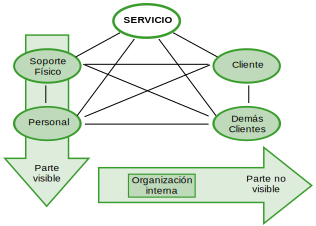
\includegraphics[width=92mm]{capitulos/graficos/procesoProductivoServiciosEiglier} 
	\label{fig:procesoProductivoServiciosEiglier} 

	\footnotesize
		Fuente: Lilian, 2004, p. 6.
\end{figure}

Y por último, hay que mencionar el margen del servicio (Eiglier y Langeard, 1976) (ver figura \ref{fig:servuccion}), que es donde confluyen todos los factores anteriormente definidos una vez que el servicio se ha desarrollado. Se trata de la suma de las ventajas competitivas conseguidas por cada factor por separado. Esto quiere decir, que el resultado del margen es lo que el cliente ha percibido, le ha gustado y ha experimentado, es decir, el vínculo real y emocional que se ha desarrollado dentro del cliente y que ha provocado una fidelización. Por ejemplo, los clientes que pertenecen al club de fidelidad que el hotel del estudio empírico propone y en el cual, se reciben descuentos, estancias en hoteles gratuitas, etc.

A modo de resumen, Eiglier y Langeard, (1976) plantean un  proceso productivo en los servicios similar al de Grönroos (2004), pero más general ya que fue desarrollado varios años antes (ver figura \ref{fig:procesoProductivoServiciosEiglier}).

Eiglier y Langeard, (1976), establecen tres tipos de ventajas competitivas: 

\begin{itemize} 
			\item La ventaja competitiva enfocada hacia la oferta total del servicio. Para poder alcanzar esta co-creación de valor deben satisfacerse las necesidades de los clientes y del personal, de los proveedores, y de todos los agentes que se encuentren implicados en la toma de decisiones como los \emph{stakeholders}. 
			\item La ventaja competitiva enfocada hacia el soporte de la oferta. Como por ejemplo, el soporte físico, el personal, la organización y la administración. 
			\item La ventaja competitiva enfocada hacia la oferta total del servicio y hacia el soporte de la oferta. Se tienen en cuenta las percepciones de antiguos clientes y en base a sus expectativas, se evalúan, aceptan e integran en el proceso productivo del servicio. Esto pone de manifiesto que el servicio global debe enfocarse a cada segmento de clientes, es decir a los denominados \emph{clientes meta}. 

\end{itemize}

En el desarrollo de los procesos de servucción, no hay que perder de vista que el cliente es la razón de ser del servicio y que las necesidades y la personalidad de los usuarios están en continua evolución, además de la heterogeneidad de cada uno de los clientes. Por lo tanto, la implementación de procesos se encuentra en cambio constante y esto supone un control y una evaluación continuada de los consumidores (Eiglier y Langeard, 1976).

Como conclusión, se puede decir que el análisis de las servucciones permite identificar el soporte físico, el personal que debe ser contratado por la empresa y la organización interna necesaria para satisfacer las expectativas de los usuarios y co-crear valor para el cliente. De este modo, se permite la identificación de aquellas actividades positivas para la empresa, otorgando la oportunidad empresarial de elaborar propuestas de cambio en las actividades conduciendo a una mejora continua de la oferta de servicios satisfaciendo al cliente y alcanzando el objetivo primordial: co-crear valor.

\subsubsection{La lógica del servicio}

La investigación desarrollada por la escuela nórdica se denomina la lógica del servicio (LS) (Grönroos, 2006). Esta corriente de pensamiento sugiere que la creación de valor se basa en la interacción de \emph{servicio por servicio}. Grönroos, argumenta que la interacción de servicio por servicio viene dada por una nueva perspectiva del cliente, mientras que el intercambio de servicios por servicios viene dada por la perspectiva de la empresa.

Por lo tanto, centrándose en la LS, Grönroos (2008) define la interacción como una acción mutua o recíproca en la que el cliente o la empresa tiene efectos uno sobre el otro y viceversa y además, de una forma simultánea, también en los procesos de creación de valor de las empresas. Grönroos, (2008) propone un modelo de productividad para los servicios que se puede visualizar a través de la figura \ref{fig:procesoProductivoServiciosGronroos} y que es más concreto que el de Eiglier y Langeard.

\begin{figure}[!h]
	\caption{El modelo de productividad en los servicios}
	\centering 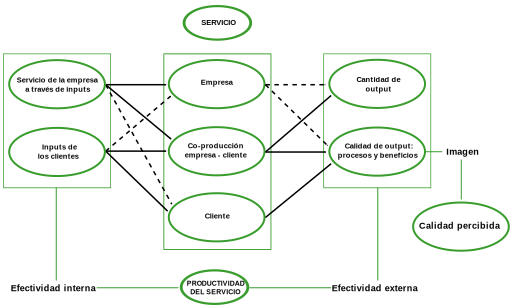
\includegraphics[width=150mm]{capitulos/graficos/procesoProductivoServiciosGronroos} 
	\label{fig:procesoProductivoServiciosGronroos} 

	\footnotesize
		Fuente: Grönroos, 2004, p. 420.
\end{figure}

Grönroos (2008) propone que las interacciones del mercado pueden extenderse más allá de las partes que están en contacto directo entre sí. Incluyendo un nuevo término que es la \emph{facilitación}. Gracias al desarrollo tecnológico existen nuevas formas de interactuar y las empresas deben facilitarlas a los clientes. Estos nuevos métodos de interacción, también influyen en los clientes abarcando novedosos sistemas de co-creación de valor en el que también se integran los recursos. Este punto de vista de que los clientes pueden ser creadores de valor difiere de la visión de la LDS de que los clientes siempre son co-creadores de valor. Como punto común, ambas lógicas reconocen la integración de los recursos como la actividad clave para la creación de valor, pero esta última incluye la interacción. Pero Grönroos (2004), en su postura más radical establece que la integración de los recursos en el proceso de co-creación de valor, puede hacer que los clientes sean los únicos capaces de crear valor. Las empresas podrían participar activamente en los procesos de creación de valor de los clientes y crear valor para los usuarios, y los clientes a su vez crear valor para sí mismos. En el anexo \ref{anexo:5} se puede encontrar más información acerca de esta cuestión.

Otro aspecto importante que resalta Grönroos (2008) en la lógica del servicio, es el cumplimiento de los esfuerzos de los clientes para concretizar y poder hacer realidad el valor. Este cumplimiento del valor es un proceso continuo donde están en juego la actualización y la realización de valor. La actualización es la percepción del cliente a la hora de recibir valor y los esfuerzos que éste emplea para que esa percepción se actualice automáticamente (ver figura \ref{fig:esferasGronroos}).

\begin{figure}[!h]
	\caption{Las esferas de la co-creación de valor en la lógica del servicio}
	\centering 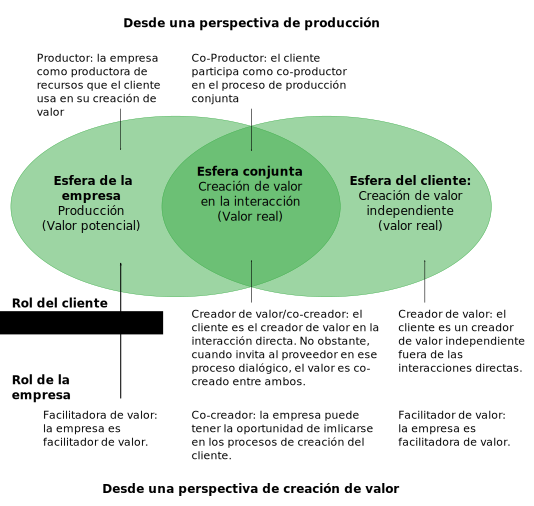
\includegraphics[width=140mm]{capitulos/graficos/esferasGronroos} 
	\label{fig:esferasGronroos} 

	\footnotesize
		Fuente: Grönroos y Voima, 2011 p. 9.
\end{figure}

En la figura \ref{fig:esferasGronroos} se puede observar cómo las funciones de la empresa y cliente varían, dependiendo de la esfera de la co-creación de valor. La empresa es la responsable del proceso de producción donde se producen los recursos y los procesos para el uso de los clientes facilitando así la creación de valor a los usuarios. Tal y como propone Grönroos (2008), si la empresa proporciona un potencial valor en uso, la empresa puede ser considerada como facilitadora de valor. En este caso, el papel del cliente es doble porque es co-creador de valor, y co-productor de los recursos y de los procesos con la empresa porque crean valor de forma conjunta con la compañía. En el momento en el que surge la interacción directa entre la empresa y el cliente, la organización puede tener la oportunidad de participar en un proceso de creación de valor del cliente y asumir el papel de co-creadora de valor. El valor puede surgir también en las otras dos esferas en diferentes períodos de tiempo, formándose así diferentes patrones de creación de valor. Puede darse que un cliente activo sea co-desarrollador o diseñador, o incluso co-fabricante, entonces la esfera conjuntase hace más grande y todo el proceso se iniciadirectamente en la esfera de valor conjunto (Grönroos y Voima, 2011).

En resumen, la lógica del servicio ve la creación de valor como una interacción directa entre los recursos propuestos por la empresa y los recursos propios del cliente y la mezcla de ambos da como resultado la creación de valor. Esta experiencia de interacciones directas hacen posible que tanto empresas como clientes sean capaces de actualizar y darse cuenta de que crean valor. Es importante destacar que este tipo de experiencias pueden ser acumuladas y compartidas en un futuro (Chen et. al., 2012).

\subsection{La co-creación de valor a través de las experiencias}

La tercera perspectiva viene de la mano de Prahalad y Ramaswamy (2004). Estos autores establecen que la co-creación de valor se da en la experiencia de los clientes a la hora del disfrute del bien o servicio, es decir, el valor no deriva del consumo de bienes y servicios, sino que está incrustado en las experiencias personalizadas y reales que se crean gracias al compromiso y la participación conjunta con la empresa. 

Es importante mencionar el momento en el que Prahalad y Ramaswamy (2004) deciden crear una nueva rama, a partir de las teorías desarrolladas hasta el momento, denominada como: la co-creación de valor en las experiencias. En la figura \ref{fig:interaccionPrahalad}, se puede apreciar como las empresas se centran en un modelo de intercambio donde la orientación es hacia el cliente y en el que se incluye este concepto de creación de valor a través de la experiencia del cliente. El valor surge en el momento en el que se produce la interacción y la comunicación entre la empresa y el cliente de una forma personalizada. El mercado es el lugar donde se intercambia el valor y el consumidor tiene que ser persuadido por la empresa para que ésta pueda percibir el máximo valor en el momento de la/s transacción/es. Los clientes están aprendiendo a estar informados, conectados, a ser autorizados por la empresa para poder realizar actividades por si solos y sobre todo a darse cuenta de que ellos también pueden recibir valor, incluso a partir del diálogo de consumidor a consumidor.

\begin{figure}[!h]
	\caption{El proceso de co-creación de valor}
	\centering 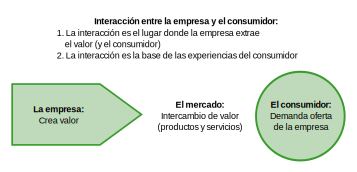
\includegraphics[width=140mm]{capitulos/graficos/interaccionPrahalad} 
	\label{fig:interaccionPrahalad} 

	\footnotesize
		Fuente: Prahalad y Ramaswamy, 2004, p. 7.
\end{figure}

Esta nueva sensación que experimentan los clientes les hace ser conscientes del poder que tienen dentro de una empresa. Por ello, un número cada vez mayor de clientes están mucho más dispuestos a negociar los precios y otras condiciones de transacción con las empresas. Prahalad y Ramaswamy (2004) afirman que la sociedad se está moviendo hacia un mundo en el que el valor es el resultado de una negociación implícita entre el consumidor individual y la empresa. 

Para subsanar el problema de la \emph{walmartización}\footnote{Concepto desarrollado en el anexo \ref{anexo:6}.}, las empresas deben de co-crear valor con los clientes a través de un enfoque obsesivo de interacciones personalizadas entre el consumidor y la empresa. Esto permitirá que los clientes se centren en las experiencias para conseguir co-crear valor. Hay que tener en cuenta el impacto que puede tener la convergencia de ambos ya que en los roles tradicionales son claramente distintos (Prahalad y Ramaswamy, 2004).

En el sistema tradicional, las empresas deciden los productos y los servicios que se producen y qué grado de valor tienen para el cliente, por lo tanto el cliente no co-crea valor. Según los autores Prahalad y Ramaswamy (2004), en las dos últimas décadas las empresas han querido otorgar mayores responsabilidades a los clientes, por ejemplo permitiendo la reserva de habitaciones por Internet. También, los usuarios pueden participar en el diseño de productos. Esto es gracias a que los consumidores están conectados, informados, capacitados y activos continuamente. Por ejemplo, en el sector hotelero existen multitud de establecimientos y algunos de ellos con grandes parecidos, pero lo que les diferencia son las experiencias que proponen al huésped, es decir, la ventaja competitiva a través de la co-creación de valor. Este ejemplo, muestra como los productos o servicios pueden ser de consumo masivo pero por el contrario, las experiencias de co-creación de valor nunca lo pueden ser. 

La co-creación de experiencias se basa principalmente en las interacciones entre la empresa y el cliente mediante el diálogo, el acceso -por ejemplo las plataformas \emph{engagement}-, el riesgo o beneficio compartido y la transparencia (Prahalad y Ramaswamy, 2004). Si se traduce al castellano la palabra \emph{engagement}, se obtendría como resultado: compromiso. Por lo tanto se trata de plataformas de compromiso entre las empresas y los clientes. Estas plataformas puede suponer un punto de contacto visual y físico de integración de recursos y de co-creación de valor. Esto quiere decir, que estas interacciones entre el consumidor y la empresa se pueden convertir en una fuente de resolución de problemas por medio del dialogo, gracias a la rapidez y eficacia del acceso a la información y también a la transparencia. Además, disminuye la incertidumbre y la toma de decisiones es más rápida. Prahalad y Ramaswamy, (2004) desarrollaron esta idea a través del modelo DART: diálogo, acceso, riesgo/beneficio y transparencia (ver figura \ref{fig:DartPrahalad}).

\begin{figure}[!h]
	\caption{El modelo DART para la co-creación de valor}
	\centering \includegraphics[width=90mm]{capitulos/graficos/DartPrahalad} 
	\label{fig:DartPrahalad} 

	\footnotesize
		Fuente: Prahalad y Ramaswamy, 2004, p. 9.
\end{figure}

A continuación, se van a explicar brevemente las variables que componen el modelo DART de Prahalad y Ramaswamy (2004) (ver figura \ref{fig:DartPrahalad}):

\begin{itemize} 
			\item \emph{El diálogo}. Es un elemento muy importante a la hora de la co-creación de valor. Implica la interactividad, la participación, la capacidad y la voluntad de actuación por parte de la empresa y por parte del cliente. Para que sea un un diálogo activo y se desarrolle favorablemente, tanto para la empresa como para el consumidor, ambos deben considerarse como iguales. La base del diálogo es abarcar temas de interés para ambos y no sobrepasar los límites establecidos. 
			\item \emph{El acceso}. Si los si los consumidores no disponen de la misma accesibilidad se vuelve al problema tradicional, donde se experimenta la asimetría de la disposición de información. 
			\item \emph{La transparencia}. Ocurre algo similar a lo explicado en el punto anterior (el acceso). Las empresas tradicionalmente casi siempre se han beneficiado de la explotación de esa asimetría de información que existía entre empresa y consumidor. Actualmente, y gracias a la conectividad, es posible que un consumidor tenga acceso a tanta información como necesite. 
			\item \emph{Los riesgos y los beneficios}. Se trata de la evaluación de la situación por parte del cliente que puede llevarle a tomar una decisión de consumo o no. Por ejemplo, si un huésped quiere volver a hospedarse en el mismo hotel y cuáles serían los riesgos de cambiar de opción. 

\end{itemize}

Las empresas se encuentran ante un reto complicado, ya que para poder llevar a cabo esta co-creación de valor a través de las interacciones de alta calidad entre el cliente y la empresa, tienen que invertir en la construcción de nuevas infraestructuras, capacidades funcionales, etc. que permitan crear una ventaja competitiva sostenible en el futuro. Las empresas que logren este objetivo, serán aquellas que pueden co-crear valor a través de experiencias únicas. (Prahalad y Ramaswamy, 2004). Aun así, hay que señalar que las compañías casi siempre han sido reticentes para dar acceso y a ser trasparentes con los clientes. Pero actualmente un número cada vez mayor está logrando estos objetivos creando infraestructuras diseñadas para llevar a cabo el diálogo entre cliente y empresa. Esto requiere de una inversión en tecnología, una inversión en la socialización de los administradores y el cambio en algunas prácticas de gestión. Los sistemas interactivos, que son los más utilizados por las compañías, permite a los consumidores expresar sus deseos y su voluntad de obtener beneficios a partir de sus propias experiencias y lo hacen explícitamente. El diálogo obliga a las empresas a invertir tiempo y esfuerzo para entender esta nueva economía de la experiencia y el desarrollo de estos nuevos sistemas permite llegar a acuerdos con rapidez estableciendo una serie de límites y negando a los consumidores algunas opciones (Prahalad y Ramaswamy, 2004) (ver figura \ref{fig:DartPrahalad}). Por otro lado, los consumidores tienen que ser conscientes de que para ellos también pueden existir riesgos y deben aceptarlo a la hora de establecer la relación de co-creación de valor. Por ejemplo, si un cliente no sabe nadar y utiliza la piscina del hotel tendrá que asumir los riesgos. La meta por ambas partes ha de ser la co-creación de valor a partir de las experiencias personalizadas de valor únicas ya que los productos y servicios personalizados van dirigidos a un cliente en particular Prahalad y Ramaswamy, (2003).

El enfoque que defienden los autores Prahalad y Ramaswamy (2004) es complejo y aporta un número importante de cambios, entre ellos, hay que tener en cuenta que cada individuo quiere interaccionar con la empresa de una forma diferente. Por ello, afirman que puede haber múltiples puntos de interacción a lo largo de la experiencia y todos ellos son fundamentales para la creación de valor. La empresa no es capaz de predecir en qué momento el consumidor va a necesitar llevar a cabo una experiencia (Prahalad y Ramaswamy, 2003).

\begin{figure}[!h]
	\caption{El mercado y la generación de valor}
	\centering 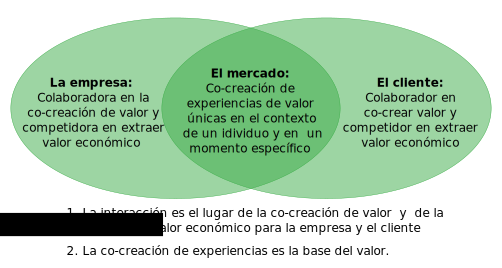
\includegraphics[width=140mm]{capitulos/graficos/esferasPrahalad} 
	\label{fig:esferasPrahalad} 

	\footnotesize
		Fuente: Prahalad y Ramaswamy, 2004, p. 11.
\end{figure}

La empresa debe centrarse en el consumidor y ha de fomentar la participación activa durante la experiencia de co-creación de valor, incluyendo la búsqueda de información, la configuración de productos y servicios, el cumplimiento y el consumo, para que las compañías puedan alcanzar las expectativas y las experiencias que los consumidores desean. (Prahalad y Ramaswamy, 2004). Por lo tanto, el mercado debe de centrarse en la convergencia de la empresa y el consumidor que da como resultado la co-creación de valor y ambos se vuelven inseparables (ver figura \ref{fig:esferasPrahalad}). Este sistema es muy exigente, pero promete ganancias sobre la eficiencia muy importantes.

Pero hay que tener en cuenta, que la empresa y el consumidor tienen una relación de colaboración pero al mismo tiempo también son competidores a la hora de co-crear valor y de obtener un beneficio económico. El mercado como un todo, se convierte en inseparable en el proceso de creación de valor, como se muestra en la figura \ref{fig:esferasPrahalad}. Hay que tener en cuenta que en los tres sectores económicos las empresas tienen como objetivo posicionarse como primera referencia en la mente del cliente cuando éste se encuentra ante la necesidad de decidirse por un producto o servicio. Las compañías que ya han conseguido ese privilegio, siguen un modelo en el que la aproximación entre lo que espera el cliente y lo que ofrece la organización, es cada vez mayor. Este enfoque pone especial énfasis en los cambios que se producen en la definición de mercado.


En resumen, Prahalad y Ramaswamy defienden que la experiencia personalizada es la base de la co-creación de valor. Pero también afirma que la integración de recursos y la interacción son necesarias en este proceso. Prahalad y Ramaswamy (2004) también defienden que el valor está incrustado en la personalidad de los individuos y no puede ser previsible por las empresas, por ello la co-creación de valor cuestiona la distinción tradicional entre la oferta y la demanda. Para que una compañía pueda ofrecer experiencias de co-creación de valor a los clientes, se ha de crear un compromiso a través de las relaciones más profundas entre ambos. Además, sostienen que el mercado debe funcionar como un foro de experiencias personalizadas donde la empresa y el cliente actúan por separado y tienen unos roles determinados. 

\subsection{Conclusiones de las teorías asociadas a la co-creación de valor}

A continuación, se va a proponer una definición propia de la co-creación de valor teniendo en cuenta que dicha co-creación de valor surge a partir de las acciones conjuntas llevadas a cabo por el cliente y por la empresa donde se supone que el individuo ha de integrar sus propios recursos y fusionarlos con los propuestos por la empresa (Vargo y Lusch, 2004). Además, ya no existen dos roles (empresa y consumidor) si no que se fusiona en uno denominado “prosumidor” (Vargo, Maglio y Akaka, 2008) ya que la empresa y el consumidor por si solos no crean valor. 

Por lo tanto, la co-creación de valor es \emph{La co-creación de valor es la interacción entre el cliente y la empresa (Grönroos, 2012) en diferentes momentos como el diseño, la producción y el consumo o disfrute del bien o servicio (Seth, Sisodia Y Sharma, 2000) integrando los recursos de ambos (Vargo y Lusch, 2004) y creando de este modo un entorno experiencial en el que los clientes puedan tener un diálogo activo para poder construir así sus propias experiencias y percepciones personalizadas (Prahalad y Ramaswamy, 2004).}

Y por último y para finalizar con el desarrollo de las principales teorías de co-creación de valor, se va a presentar el cuadro \ref{tab:comparativaTeorias} que resume las diferencias básicas entre las teorías anteriormente expuestas que son: la lógica dominante del producto, la lógica dominante del servicio, la lógica del servicio, la servucción y la co-creación de experiencias.

%\newgeometry{left=1cm}
\begin{landscape}
\begin{table}[h]
    \caption {Comparativa de las teorías asociadas a la co-creación de valor.}
	\label{tab:comparativaTeorias}
	\setlength\extrarowheight{5pt}
	
	\begin{tabular}{p{1.8cm} p{3.8cm} p{3.8cm} p{3.8cm} p{3.8cm} p{3.8cm} }
	\toprule
		                 & LDP                                                                      & LDS                                       & LS                                       & Servucción                                                                                    & Experiencias                                                          \\ \midrule
	El valor             & Valor en el intercambio.                                                 & Valor en el contexto.                     & Valor en uso a partir de la interacción. & La co-creación de valor se realiza entre la empresa y el cliente.                             & Valor en la experiencia.                                              \\
	El cliente           & Usa y destruye el valor que ha creado la empresa a través del consumo. & Co-creador de valor.                      & Creador y co-creador de valor.           & Es productor y consumidor.                                                                    & Creador de valor a través de co-creación de experiencias.             \\
	El rol de la empresa & Produce y distribuye valor.                                              & Realiza proposiciones de valor.           & Facilitadora o realizadora de valor.     & Cuida el soporte físico, los recursos humanos y la administración y organización.             & Facilitadora de entornos de experiencias o de plataformas engagement. \\
	El servicio          & Practicamente inexistente                                                & Da solución o aplicación de competencias. & Es la actividad.                         & Sin cliente no existe el servicio.                                                            & Experiencias personalizadas.                                          \\
	Los recursos         & Unidades de output y recursos operandos.                                 & Operantes y operandos.                    & Recursos y procesos de apoyo.            & Ventajas competitivas enfocadas hacia la oferta total, hacia el soporte de la oferta o ambas. & DART: diálogo, acceso, riesgo y beneficio y transparencia.            \\ \bottomrule
	\end{tabular}

	\center
	\footnotesize
	Fuente: Adaptado de Blasco, 2014. p. 61.
\end{table}
\end{landscape}

